\documentclass[9pt]{beamer}
\usepackage[utf8x]{inputenc}
\usepackage{hyperref}
\usepackage{fontawesome}
\usepackage{graphicx}
\usepackage[english]{babel}

% ------------------------------------------------------------------------------
% Use the beautiful metropolis beamer template
% ------------------------------------------------------------------------------
\usepackage[T1]{fontenc}
\usepackage{fontawesome}
\usepackage{FiraSans} 
\mode<presentation>
{
  \usetheme[progressbar=foot,numbering=fraction,background=light]{metropolis} 
  \usecolortheme{default} % or try albatross, beaver, crane, ...
  \usefonttheme{default}  % or try serif, structurebold, ...
  \setbeamertemplate{navigation symbols}{}
  \setbeamertemplate{caption}[numbered]
  %\setbeamertemplate{frame footer}{My custom footer}
} 

% ------------------------------------------------------------------------------
% beamer doesn't have texttt defined, but I usually want it anyway
% ------------------------------------------------------------------------------
\let\textttorig\texttt
\renewcommand<>{\texttt}[1]{%
  \only#2{\textttorig{#1}}%
}

% ------------------------------------------------------------------------------
% minted
% ------------------------------------------------------------------------------
\usepackage{minted}


% ------------------------------------------------------------------------------
% tcolorbox / tcblisting
% ------------------------------------------------------------------------------
\usepackage{xcolor}
\definecolor{codecolor}{HTML}{FFC300}

\usepackage{tcolorbox}
\tcbuselibrary{most,listingsutf8,minted}

\tcbset{tcbox width=auto,left=1mm,top=1mm,bottom=1mm,
right=1mm,boxsep=1mm,middle=1pt}

\newtcblisting{myr}[1]{colback=codecolor!5,colframe=codecolor!80!black,listing only, 
minted options={numbers=left, style=tcblatex,fontsize=\tiny,breaklines,autogobble,linenos,numbersep=3mm},
left=5mm,enhanced,
title=#1, fonttitle=\bfseries,
listing engine=minted,minted language=r}


% ------------------------------------------------------------------------------
% Listings
% ------------------------------------------------------------------------------
\definecolor{mygreen}{HTML}{37980D}
\definecolor{myblue}{HTML}{0D089F}
\definecolor{myred}{HTML}{98290D}

\usepackage{listings}

% the following is optional to configure custom highlighting
\lstdefinelanguage{XML}
{
  morestring=[b]",
  morecomment=[s]{<!--}{-->},
  morestring=[s]{>}{<},
  morekeywords={ref,xmlns,version,type,canonicalRef,metr,real,target}% list your attributes here
}

\lstdefinestyle{myxml}{
language=XML,
showspaces=false,
showtabs=false,
basicstyle=\ttfamily,
columns=fullflexible,
breaklines=true,
showstringspaces=false,
breakatwhitespace=true,
escapeinside={(*@}{@*)},
basicstyle=\color{mygreen}\ttfamily,%\footnotesize,
stringstyle=\color{myred},
commentstyle=\color{myblue}\upshape,
keywordstyle=\color{myblue}\bfseries,
}


% ------------------------------------------------------------------------------
% The Document
% ------------------------------------------------------------------------------
\title{Boat Listings Newsletter}
\author{Fátima Rosa}
\date{December 10, 2021}

\begin{document}

\maketitle


\begin{frame}[fragile]{Introduction}
\alert{Business Problem}

We are developing a weekly newsletter to track market trends help sellers get more views on their boats.

We want to know which features popular boats have in common, and in specific if expensive boats are more popular.

\alert{Methodology}

We have access to the number of views of 9888 boat listings for the last 7 days.

We will select the boat listings that account for 10\% (150 boat listings) of the total number of views and analyze which features they have in common. We will also analyse how the selected listings compare with the others, e.g. in terms of price.

We will provide the marketing team with the most common features of popular boat listings, as well as identify the countries where we anticipate a better reception of our newsletter.

\end{frame}

\begin{frame}[fragile]{How price and age affect popularity?}

\begin{columns}
\begin{column}{0.5\textwidth}
    \begin{center}
     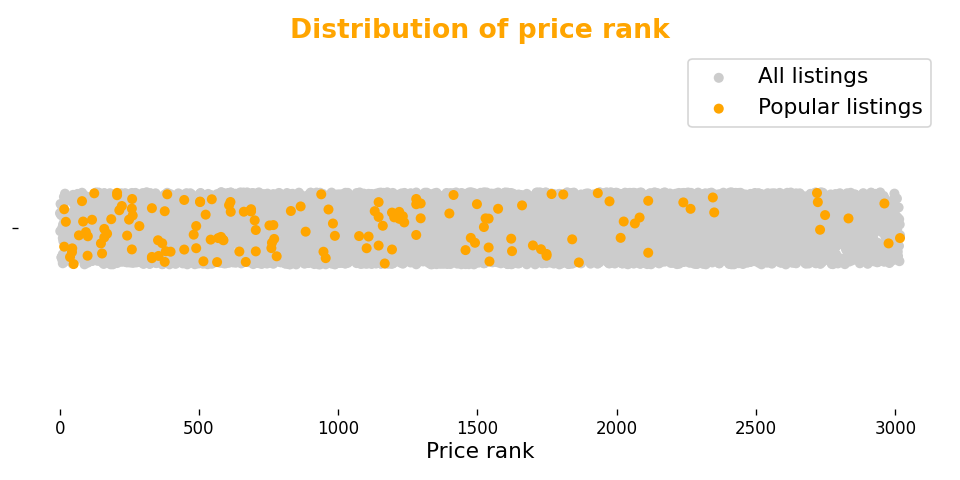
\includegraphics[width=\textwidth]{images/Price_rank.png}
     
     \vspace{1.2cm}
     
     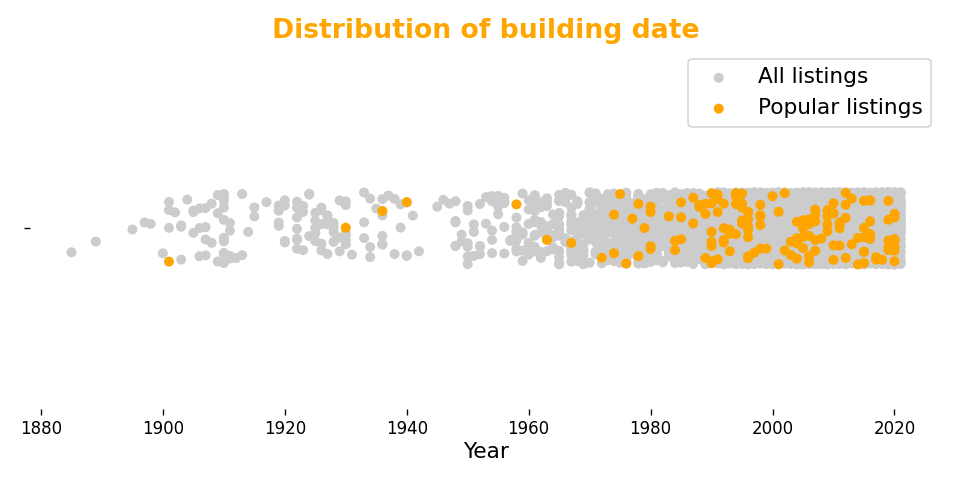
\includegraphics[width=\textwidth]{images/Year Built.png}     
    \end{center}
\end{column}
\begin{column}{0.5\textwidth}

    The \textbf{86 out of the 150 most popular listings are among the 1000th cheapest} (less than 48.864 euros).
    However, \textbf{there is not a direct connection}. For example:
    
    \begin{table}[]
        \centering
        \begin{tabular}{l l}
            \textbf{Views rank} &  \textbf{Price rank} \\
            1st &  259th \\
            2nd & 687nd \\
            3rd & 1748th \\
            4th & 2730th \\
            5th & 377th \\
        \end{tabular}
    \end{table}
    
    \textbf{The 150 most popular listings have all been built during the 20th and 21st centuries, with most having been built after 1980.}
\end{column}
\end{columns}
\end{frame}

\begin{frame}[fragile]{How length and width affect popularity?}

\begin{columns}
\begin{column}{0.5\textwidth}
    \begin{center}
     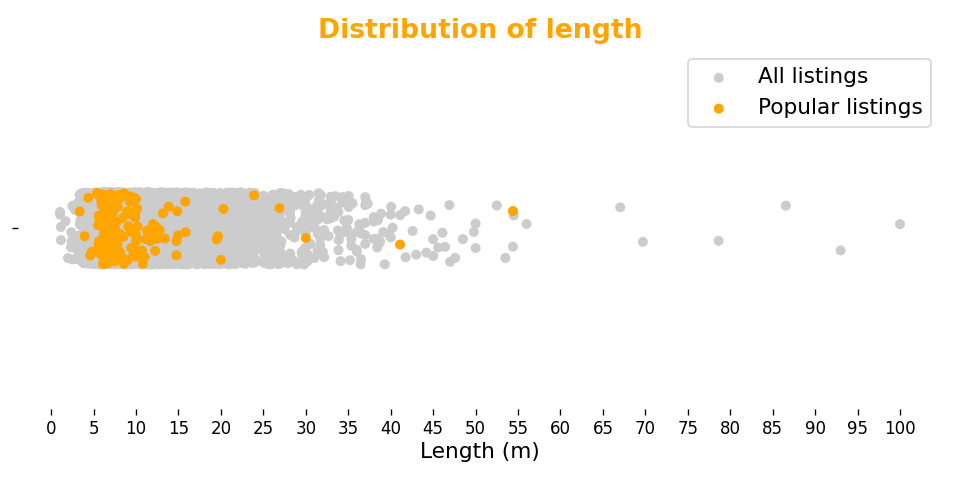
\includegraphics[width=\textwidth]{images/Length.png}
     
     \vspace{1.2cm}
     
     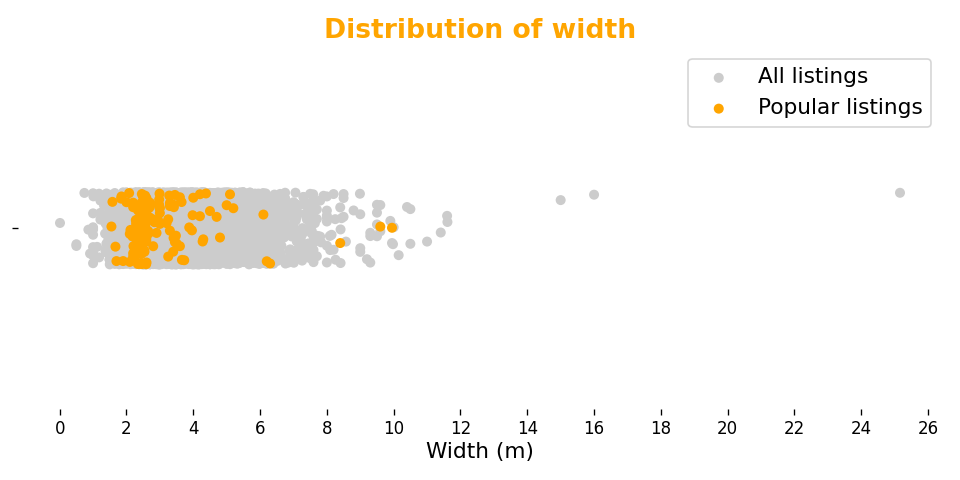
\includegraphics[width=\textwidth]{images/Width.png}     
    \end{center}
\end{column}
\begin{column}{0.5\textwidth}  %%<--- here
    Users search mostly boats with \textbf{lengths between 5 and 15 metres} and \textbf{widths between 2 and 4 metres}.
\end{column}
\end{columns}
\end{frame}

\begin{frame}[fragile]{What brands and materials are more popular?}
\begin{columns}
\begin{column}{0.5\textwidth}
    \begin{center}
     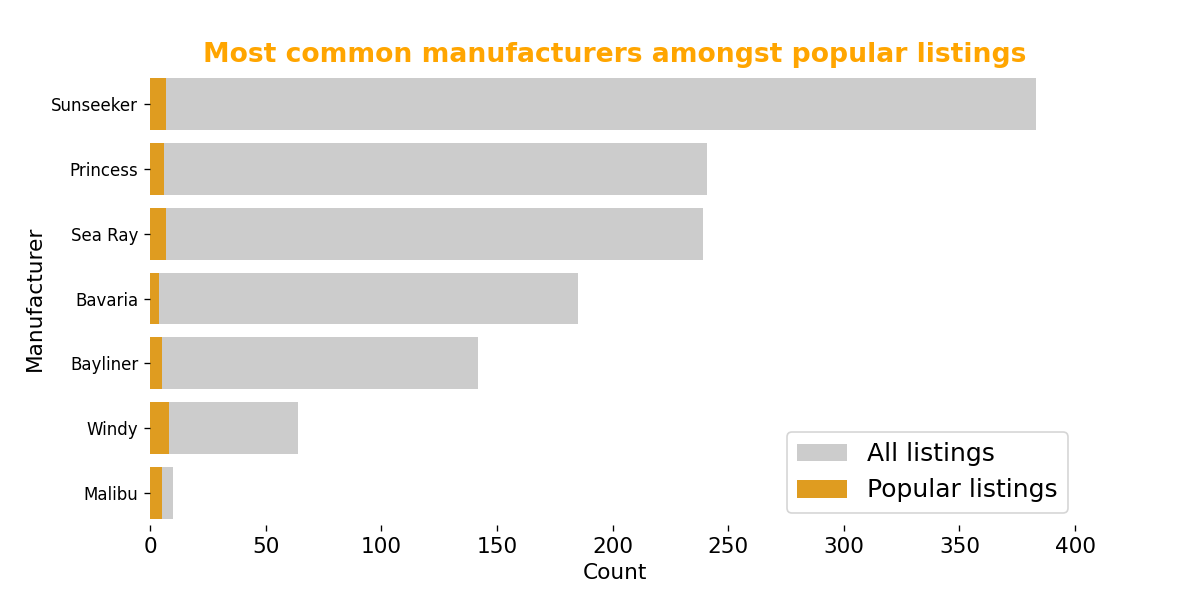
\includegraphics[width=\textwidth]{images/manufacturer.png}
     
     \vspace{1.2cm}
     
     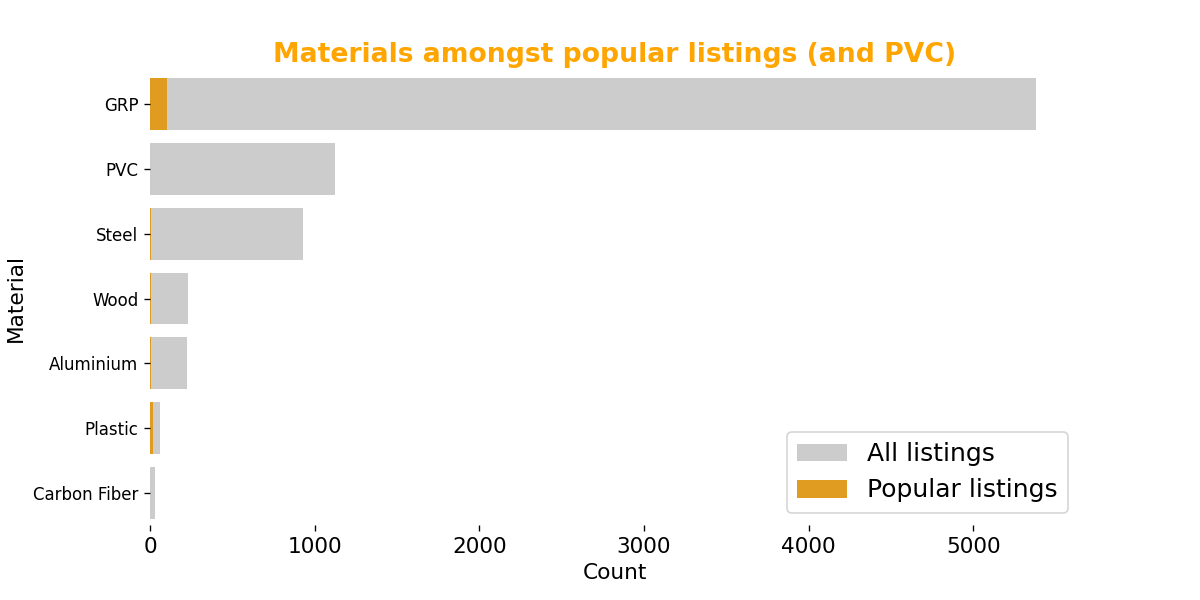
\includegraphics[width=\textwidth]{images/material.png}     
    \end{center}
\end{column}
\begin{column}{0.5\textwidth}  %%<--- here
    Amongst the \textbf{150 most popular} listings there are only \textbf{80 manufacturers}, of which only \textbf{7 have 3 or more popular listings}.
    \textbf{Despite having less listings}, manufacturers like Malibu and Windy \textbf{have as many popular listings} as Sunseeker.
    
    \vspace{.5cm}
    
    Regarding material, \textbf{most boats listed are made of GRP and most popular listings include this material}.
    Still, \textbf{Aluminum and Plastic are also popular}. 
    
    \textbf{None of the 150 most popular boat listings are made of PVC}, despite the high number of listings.
 
\end{column}
\end{columns}
\end{frame}

\begin{frame}[fragile]{What boat types and sale conditions are more popular?}
\begin{columns}
\begin{column}{0.5\textwidth}
    \begin{center}
     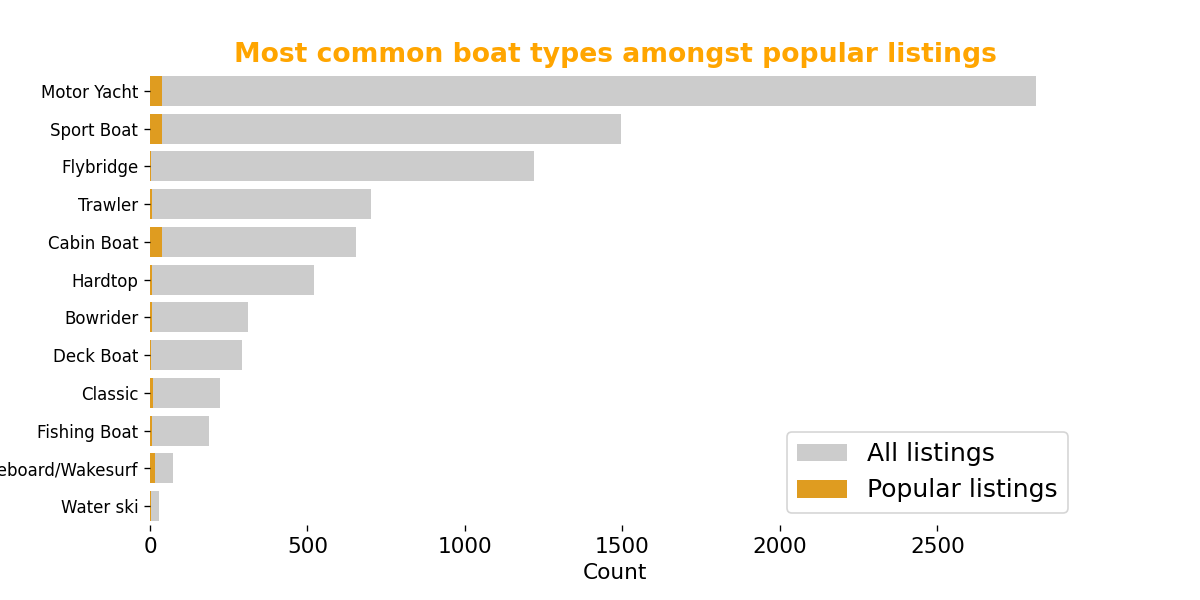
\includegraphics[width=\textwidth]{images/boat_type.png}
     
     \vspace{1.2cm}
     
     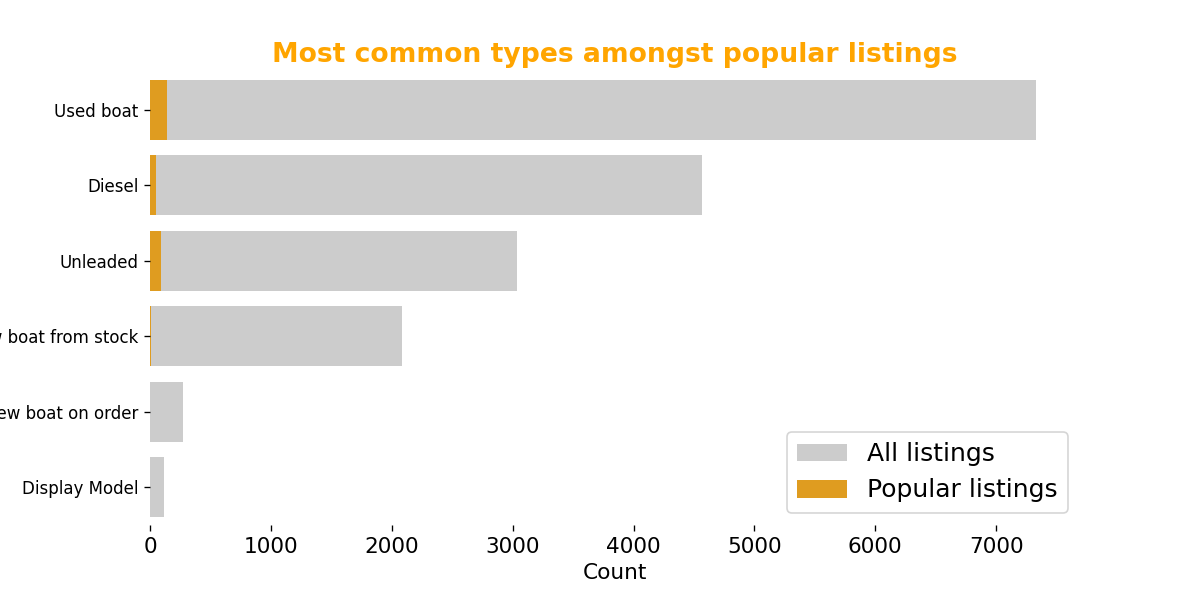
\includegraphics[width=\textwidth]{images/type.png}     
    \end{center}
\end{column}
\begin{column}{0.5\textwidth}  %%<--- here
    Amongst the \textbf{150 most popular listings} there are only \textbf{18 types of boats}, of which only \textbf{12 have 3 or more popular listings}.
    
    \textbf{Cabin Boat, Motor Yacht and Sport Boat are the most researched.}
    
    \vspace{.5cm}
    
    \textbf{Most users search for used boats and unleaded.}
 
\end{column}
\end{columns}
\end{frame}

\begin{frame}[fragile]{Countries with most views}
\begin{center}
  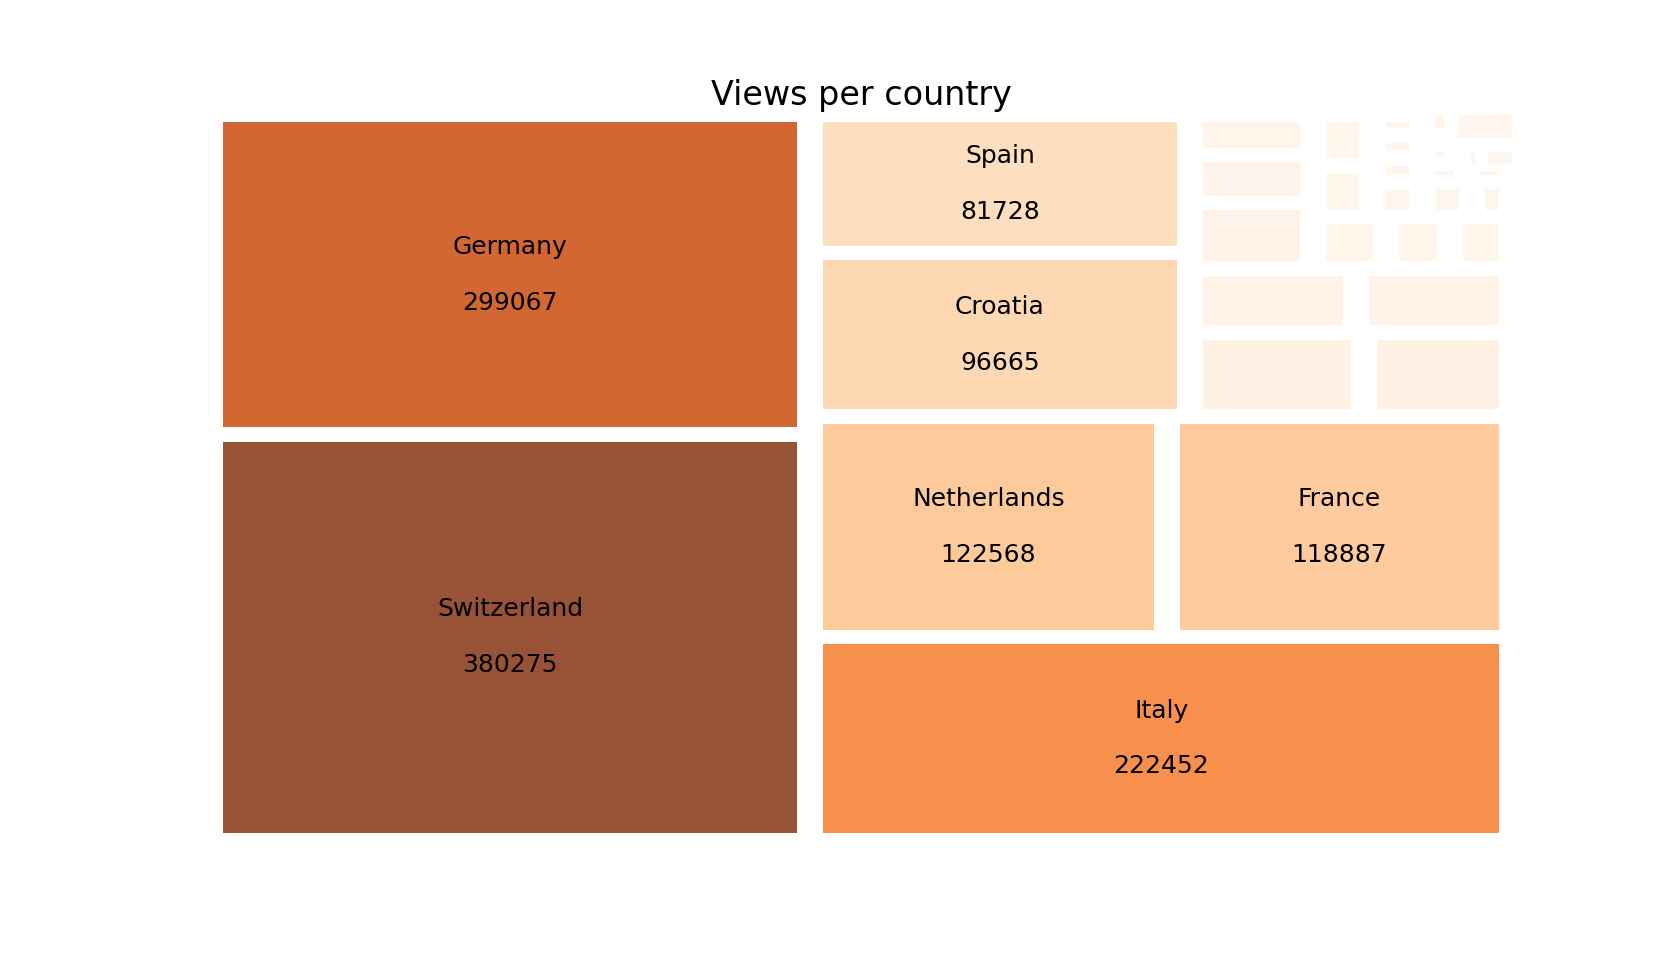
\includegraphics[width=\textwidth]{images/country.png}  
  
  \textbf{The countries with the most views are all in Central Europe.}
\end{center}



\end{frame}



\begin{frame}[fragile]{Conclusions}
The most popular listings have the following characteristics:
    \begin{itemize}
        \item Have been \textbf{built after 1980};
        \item Are relatively \textbf{small boats, with lengths between 5 and 15 metres and 
        widths between 2 and 4 metres};
        \item Are \textbf{made of GRP, aluminum or plastic};
        \item Are \textbf{cabin boats, motor yachts and/or sport boats};
        \item Are \textbf{used boats and/or unleaded}.
    \end{itemize}
    
    \textbf{Price does not seem to directly affect the number of views.}
    
    \textbf{Our newsletter will probably be more successful in Central Europe.}
    

\end{frame}

\end{document}
